\documentclass[tikz,border=0pt]{standalone}
\usepackage{fontspec}
\newlength{\cardwidth}
\newlength{\cardheight}
\setlength{\cardwidth}{60mm}
\setlength{\cardheight}{102.86mm}
\begin{document}
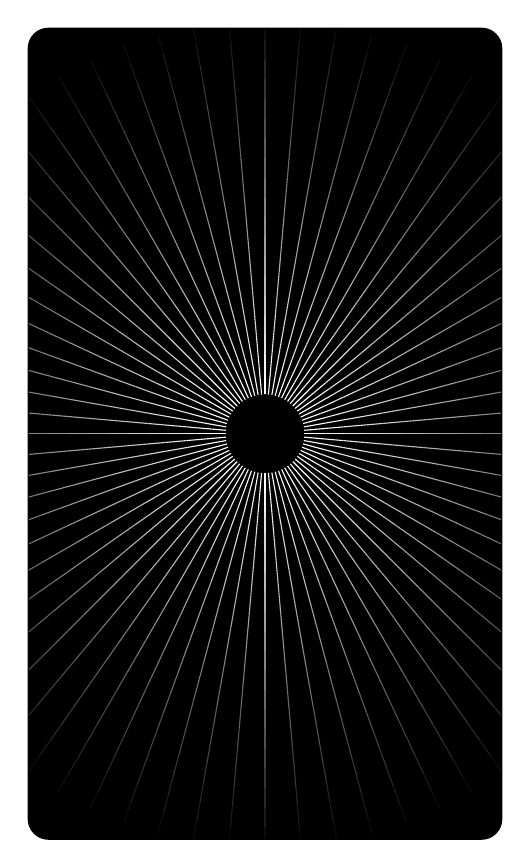
\begin{tikzpicture}
  \draw[rounded corners=2.5mm, thick] (0,0) rectangle (\cardwidth, \cardheight);
  \clip[rounded corners=2.5mm] (0,0) rectangle (\cardwidth, \cardheight);
  \fill[black] (0,0) rectangle (\cardwidth, \cardheight);
  \foreach \a in {0,5,...,355} {
    \foreach \s in {0,1,...,19} {
      \pgfmathsetmacro{\op}{1 - \s/19}%
      \pgfmathsetmacro{\startrad}{5 + \s*2.5}%
      \draw[white, thin, opacity=\op]
        (0.5\cardwidth, 0.5\cardheight) ++(\a:\startrad mm) -- ++(\a:2.5mm);
    }
  }
\end{tikzpicture}
\end{document}
